\chapter{Transform image compression}

\section{Problem statement}

\begin{enumerate}[(a)]
    \item Investigate image compression based on DCT.
          Divide the image into 8-by-8 subimages, compute the two-dimensional discrete cosine
          transform of each subimage, compress the test image to different qualities by
          discarding some DCT coefficients based on zonal mask
          and threshold mask and using the inverse discrete cosine
          transform with fewer transform coefficients. Display the
          original image, the reconstructed images and the
          difference images.

    \item Investigate image compression based on wavelets. \\
          Consider four types of wavelets:
          \begin{enumerate}
            \item Haar (2x2)
            \item Daubechies (8-tap)
            \item Symlet (8-tap)
            \item Cohen-Daubechies-Feauveau (17-tap)
          \end{enumerate}
\end{enumerate}

\section{Python implementation}
\bigskip
Two programs: \\
\begin{itemize}

    \item DCT compression: \textbf{dct.py}
    Usage:~\textbf{dct.py [-h] [--zonal | --threshold] [-z Z] image\_path} \\
    Use \textbf{python dct.py -h} to see the help.

    \bigskip

    \item Wavelet compression: \textbf{wavelet.py}
    Usage:~\textbf{wavelets.py [-h] [--haar | --daub | --symlet | --cohen] [-l LEVEL]}\\
                   \textbf{[-t THRESHOLD] image\_path}
    Use \textbf{python wavelets.py -h} to see the help.

\end{itemize}

\bigskip

\pagebreak

\begin{figure}[!htb]\centering
    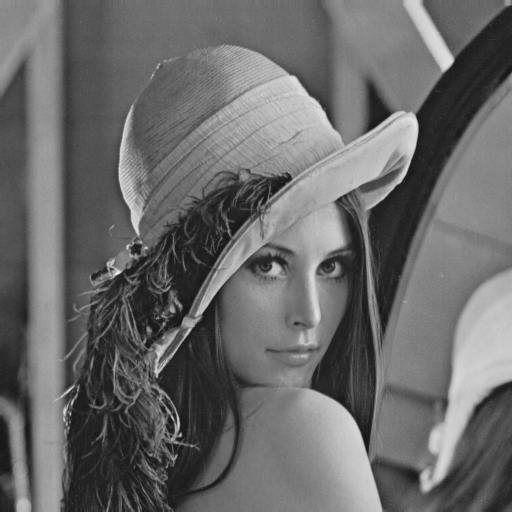
\includegraphics[width=0.6\linewidth]{./images/7/original.jpg}
    \caption{\small{Original image}}
\end{figure}

\pagebreak

\section{Image compression based on DCT}

\subsection{Zonal mask}

\textbf{python dct.py --zonal -z Z lenna.tif} where $Z = 1, 4$ or $7$.
\newline
\newline
Example: Zonal 5
\begin{equation}
\begin{bmatrix}
       1 & 1 & 1 & 1 & 1 & 0 & 0 & 0 \\
       1 & 1 & 1 & 1 & 0 & 0 & 0 & 0 \\
       1 & 1 & 1 & 0 & 0 & 0 & 0 & 0 \\
       1 & 1 & 0 & 0 & 0 & 0 & 0 & 0 \\
       1 & 0 & 0 & 0 & 0 & 0 & 0 & 0 \\
       0 & 0 & 0 & 0 & 0 & 0 & 0 & 0 \\
       0 & 0 & 0 & 0 & 0 & 0 & 0 & 0 \\
       0 & 0 & 0 & 0 & 0 & 0 & 0 & 0 \\
\end{bmatrix}
\end{equation}
\bigskip
Example: Zonal 2
\begin{equation}
\begin{bmatrix}
       1 & 1 & 0 & 0 & 0 & 0 & 0 & 0 \\
       1 & 0 & 0 & 0 & 0 & 0 & 0 & 0 \\
       0 & 0 & 0 & 0 & 0 & 0 & 0 & 0 \\
       0 & 0 & 0 & 0 & 0 & 0 & 0 & 0 \\
       0 & 0 & 0 & 0 & 0 & 0 & 0 & 0 \\
       0 & 0 & 0 & 0 & 0 & 0 & 0 & 0 \\
       0 & 0 & 0 & 0 & 0 & 0 & 0 & 0 \\
       0 & 0 & 0 & 0 & 0 & 0 & 0 & 0 \\
\end{bmatrix}
\end{equation}

\begin{figure}[!htb]\centering
    \begin{minipage}{0.45\textwidth}
        \frame{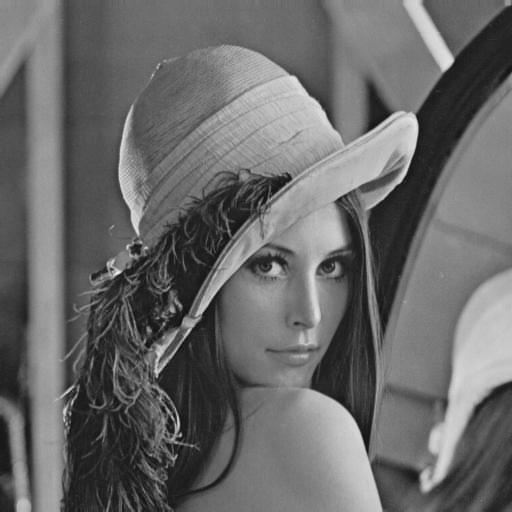
\includegraphics[width=\linewidth]{./images/7/dct_zonal_7.jpg}}
        \caption{\small{Zonal 7}}
    \end{minipage}
    \begin{minipage}{0.45\textwidth}
        \frame{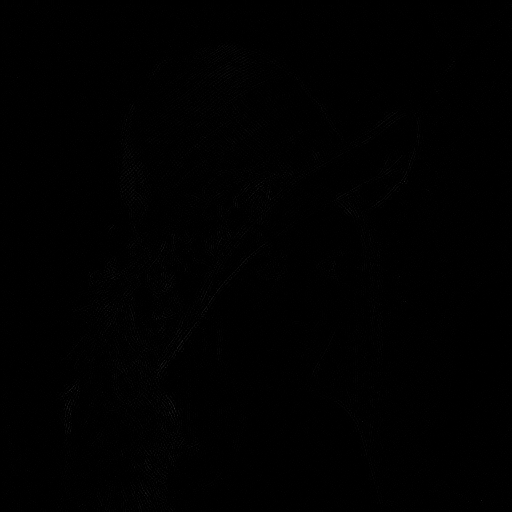
\includegraphics[width=\linewidth]{./images/7/dct_zonal_7_diff.jpg}}
        \caption{\small{Zonal 7 - Diff}}
    \end{minipage}
\end{figure}

\pagebreak

\begin{figure}[!htb]\centering
    \begin{minipage}{0.4\textwidth}
        \frame{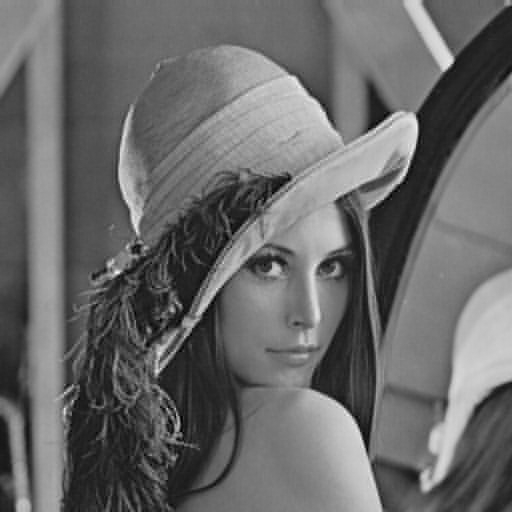
\includegraphics[width=\linewidth]{./images/7/dct_zonal_4.jpg}}
        \caption{\small{Zonal 4}}
    \end{minipage}
    \begin{minipage}{0.4\textwidth}
        \frame{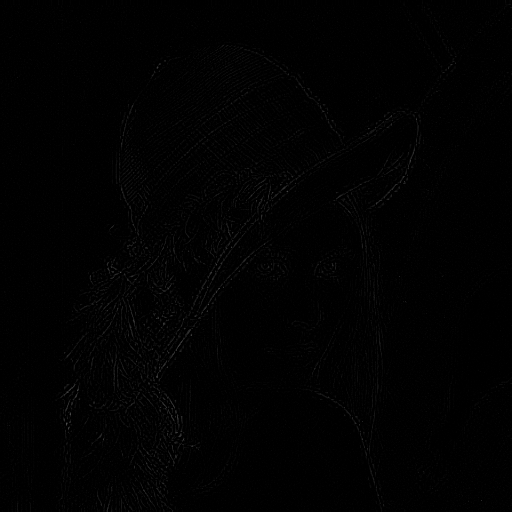
\includegraphics[width=\linewidth]{./images/7/dct_zonal_4_diff.jpg}}
        \caption{\small{Zonal 4 - Diff}}
    \end{minipage}
\end{figure}

\begin{figure}[!htb]\centering
    \begin{minipage}{0.4\textwidth}
        \frame{
\includegraphics[width=\linewidth]{./images/7/dct_zonal_2.jpg}}
        \caption{\small{Zonal 2}}
    \end{minipage}
    \begin{minipage}{0.4\textwidth}
        \frame{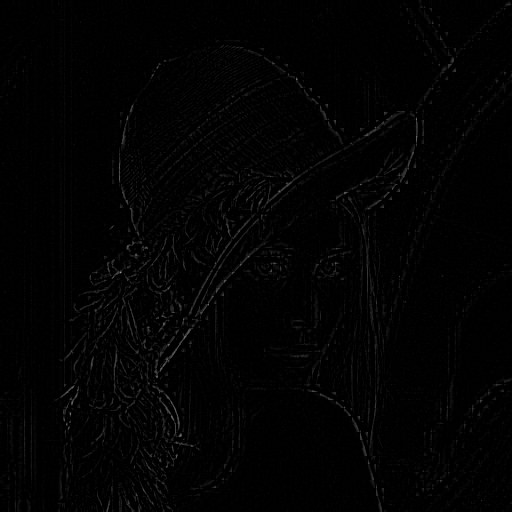
\includegraphics[width=\linewidth]{./images/7/dct_zonal_2_diff.jpg}}
        \caption{\small{Zonal 2 - Diff}}
    \end{minipage}
\end{figure}


\begin{figure}[!htb]\centering
    \begin{minipage}{0.4\textwidth}
        \frame{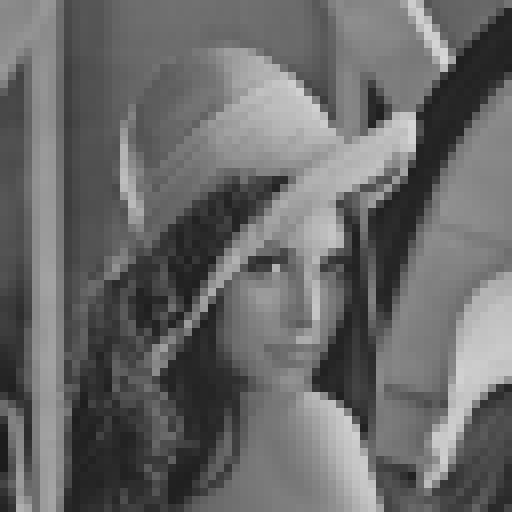
\includegraphics[width=\linewidth]{./images/7/dct_zonal_1.jpg}}
        \caption{\small{Zonal 1}}
    \end{minipage}
    \begin{minipage}{0.4\textwidth}
        \frame{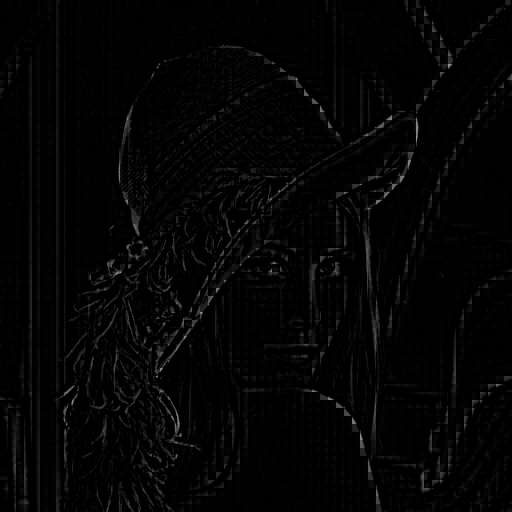
\includegraphics[width=\linewidth]{./images/7/dct_zonal_1_diff.jpg}}
        \caption{\small{Zonal 1 - Diff}}
    \end{minipage}
\end{figure}

\pagebreak

\section{Image compression based on Wavelets}

Decompose the image by wavelets, truncate some coefficients to 0 below a threshold (0 in this case) and reconstructed the image.\\
\textbf{python wavelets.py --haar lenna.tif -l 1 -t 0}.

\pagebreak
\subsection{Haar}

\begin{figure}[!htb]\centering
    \begin{minipage}{0.8\textwidth}
        \frame{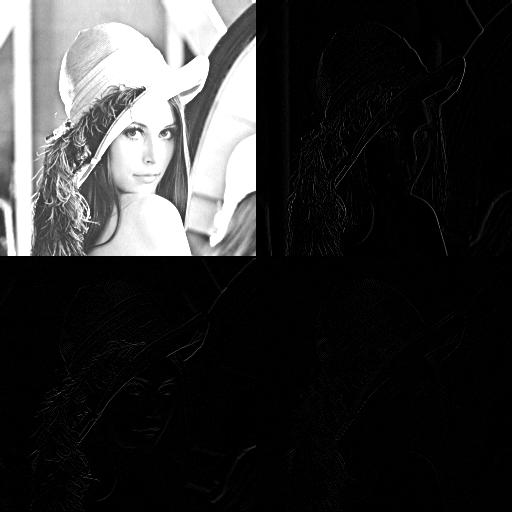
\includegraphics[width=\linewidth]{./images/7/haar.jpg}}
        \caption{\small{Haar}}
    \end{minipage}
\end{figure}

\begin{figure}[!htb]\centering
    \begin{minipage}{0.45\textwidth}
        \frame{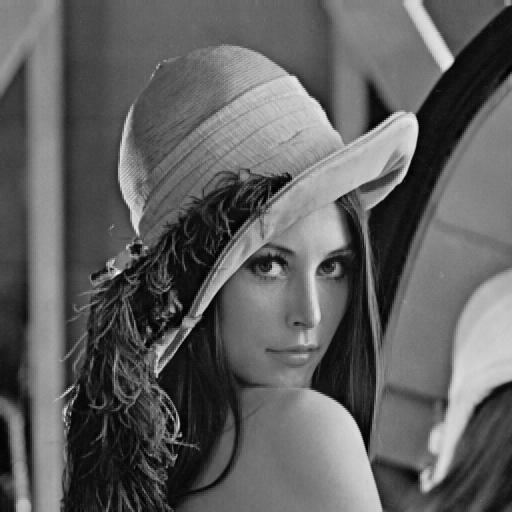
\includegraphics[width=\linewidth]{./images/7/haar_reconstructed.jpg}}
        \caption{\small{Haar reconstructed}}
    \end{minipage}
    \begin{minipage}{0.45\textwidth}
        \frame{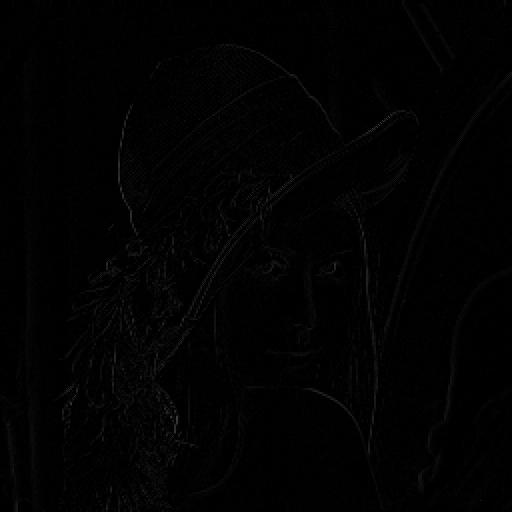
\includegraphics[width=\linewidth]{./images/7/haar_diff.jpg}}
        \caption{\small{Haar difference}}
    \end{minipage}
\end{figure}

\pagebreak
\subsection{Daubechies}

\begin{figure}[!htb]\centering
    \begin{minipage}{0.8\textwidth}
        \frame{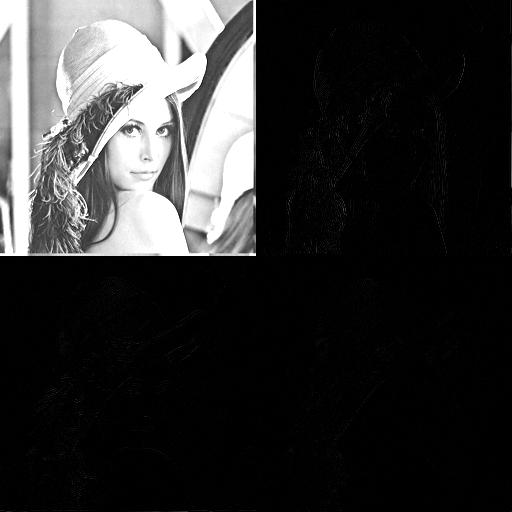
\includegraphics[width=\linewidth]{./images/7/daub.jpg}}
        \caption{\small{Daubechies}}
    \end{minipage}
\end{figure}

\begin{figure}[!htb]\centering
    \begin{minipage}{0.45\textwidth}
        \frame{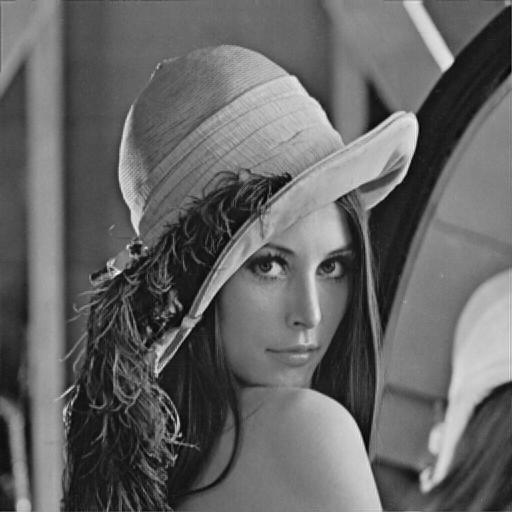
\includegraphics[width=\linewidth]{./images/7/daub_reconstructed.jpg}}
        \caption{\small{Daubechies reconstructed}}
    \end{minipage}
    \begin{minipage}{0.45\textwidth}
        \frame{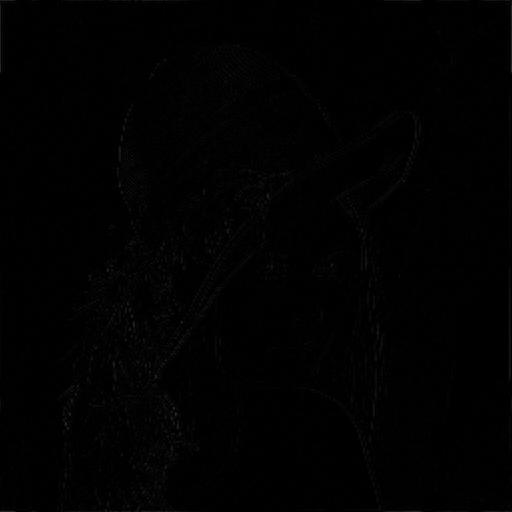
\includegraphics[width=\linewidth]{./images/7/daub_diff.jpg}}
        \caption{\small{Daubechies difference}}
    \end{minipage}
\end{figure}

\pagebreak
\subsection{Symlet}

\begin{figure}[!htb]\centering
    \begin{minipage}{0.8\textwidth}
        \frame{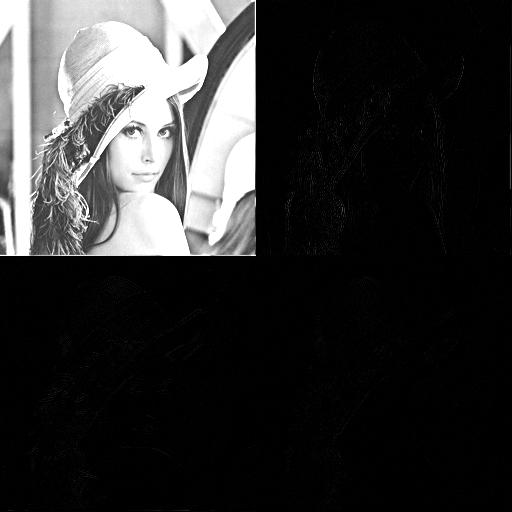
\includegraphics[width=\linewidth]{./images/7/symlet.jpg}}
        \caption{\small{Symlet}}
    \end{minipage}
\end{figure}

\begin{figure}[!htb]\centering
    \begin{minipage}{0.45\textwidth}
        \frame{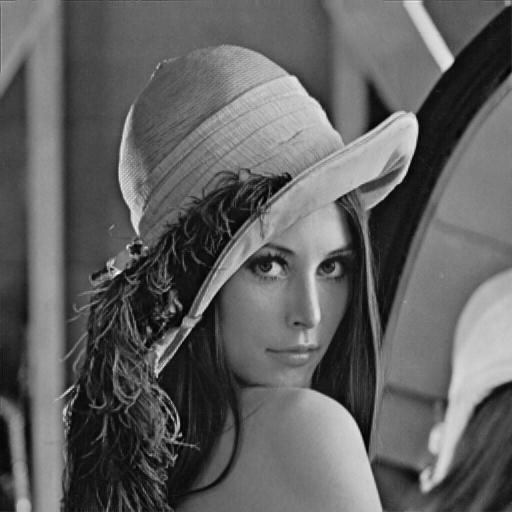
\includegraphics[width=\linewidth]{./images/7/symlet_reconstructed.jpg}}
        \caption{\small{Symlet reconstructed}}
    \end{minipage}
    \begin{minipage}{0.45\textwidth}
        \frame{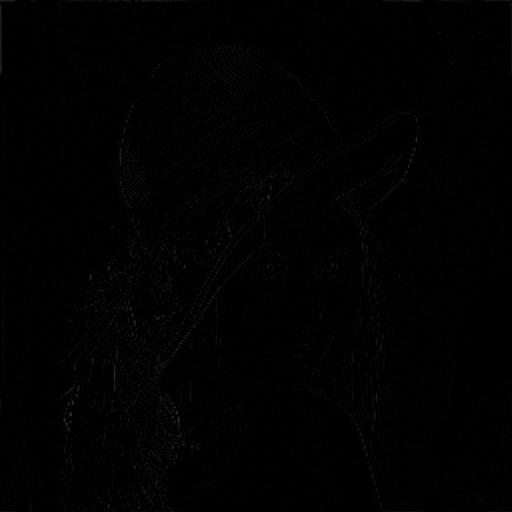
\includegraphics[width=\linewidth]{./images/7/symlet_diff.jpg}}
        \caption{\small{Symlet difference}}
    \end{minipage}
\end{figure}


\pagebreak
\subsection{Cohen-Daubechies-Feauveau}

\begin{figure}[!htb]\centering
    \begin{minipage}{0.8\textwidth}
        \frame{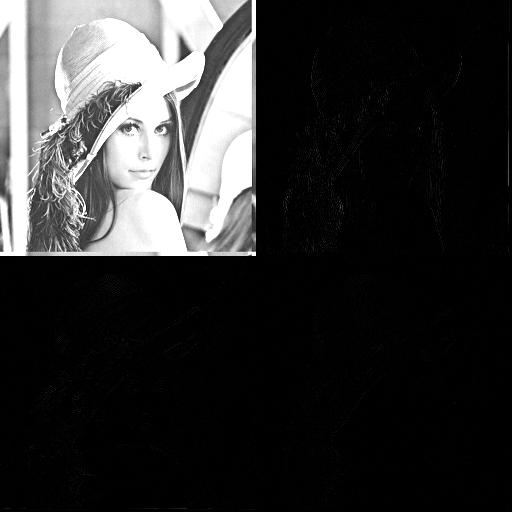
\includegraphics[width=\linewidth]{./images/7/cohen.jpg}}
        \caption{\small{Cohen}}
    \end{minipage}
\end{figure}

\begin{figure}[!htb]\centering
    \begin{minipage}{0.45\textwidth}
        \frame{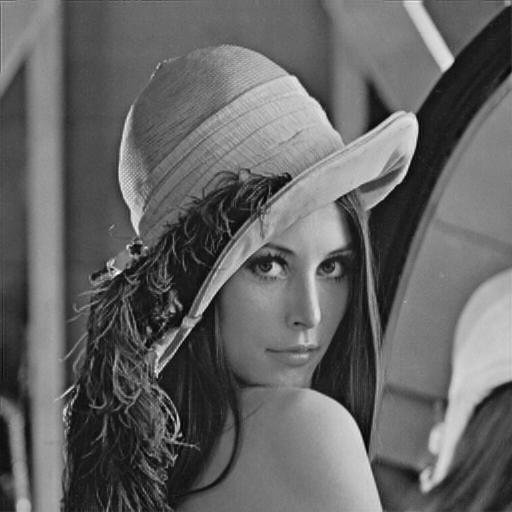
\includegraphics[width=\linewidth]{./images/7/cohen_reconstructed.jpg}}
        \caption{\small{Cohen reconstructed}}
    \end{minipage}
    \begin{minipage}{0.45\textwidth}
        \frame{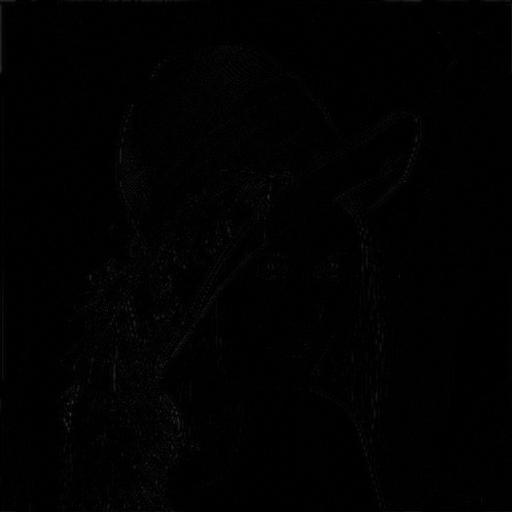
\includegraphics[width=\linewidth]{./images/7/cohen_diff.jpg}}
        \caption{\small{Cohen difference}}
    \end{minipage}
\end{figure}
